\documentclass[hyperref,UTF8]{ctexart}
\usepackage{CJK}
\usepackage{indentfirst}
\usepackage{amsfonts}
\usepackage{amsmath}
\usepackage{amssymb}
\usepackage{amsthm}
\usepackage{graphicx}
\usepackage{geometry}
\usepackage{titlesec}
\usepackage[colorlinks, citecolor=black,hyperfootnotes=true]{hyperref}
\usepackage{fancyhdr}
\usepackage{setspace}
\begin{document}
\title{Calculator++ Report}
\author{Li Xiang 2016011267 \\ Zhang Xilin 2016050022}
\date{July 28, 2017}
\maketitle

\vspace {2cm}
\begin{center}

\includegraphics{icon.png}
\end{center}

\newpage

\tableofcontents

\newpage

\section{发布链接}

首先我们将所有源代码以及所有用到的数据用Github以保存并合同协作。

完成的产品我们将之发布在 http://Break.github.io

\newpage

\section{功能实现}

\subsection{主题界面}
每当刷新页面会出现如下的主界面
\begin{center}
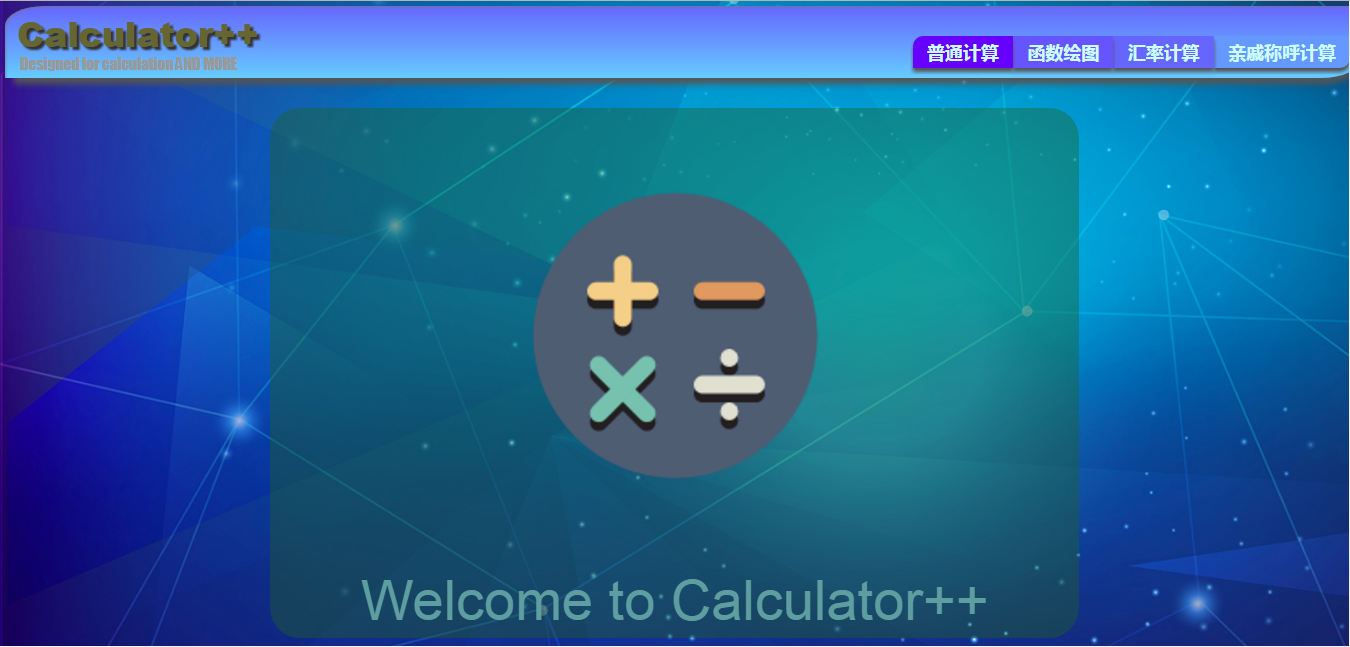
\includegraphics[width=5in]{theme.PNG}
\end{center}

在主界面的右上方有4个可以点击的选项,分别对应了计算器(融合了初等函数等),函数绘图,实时汇率计算以及亲戚关系计算器。显示界面均如下所示:

\subsection{页面切换}
每次点击四个功能选项后会调用JS函数来使其转变的更加柔和,渐隐渐现的效果。

\subsection{响应式设计}

HTML的设计采用了响应式设计,可以自适应浏览器大小并改变内容大小及位置。

\subsection{计算器}
界面如下:

\begin{center}
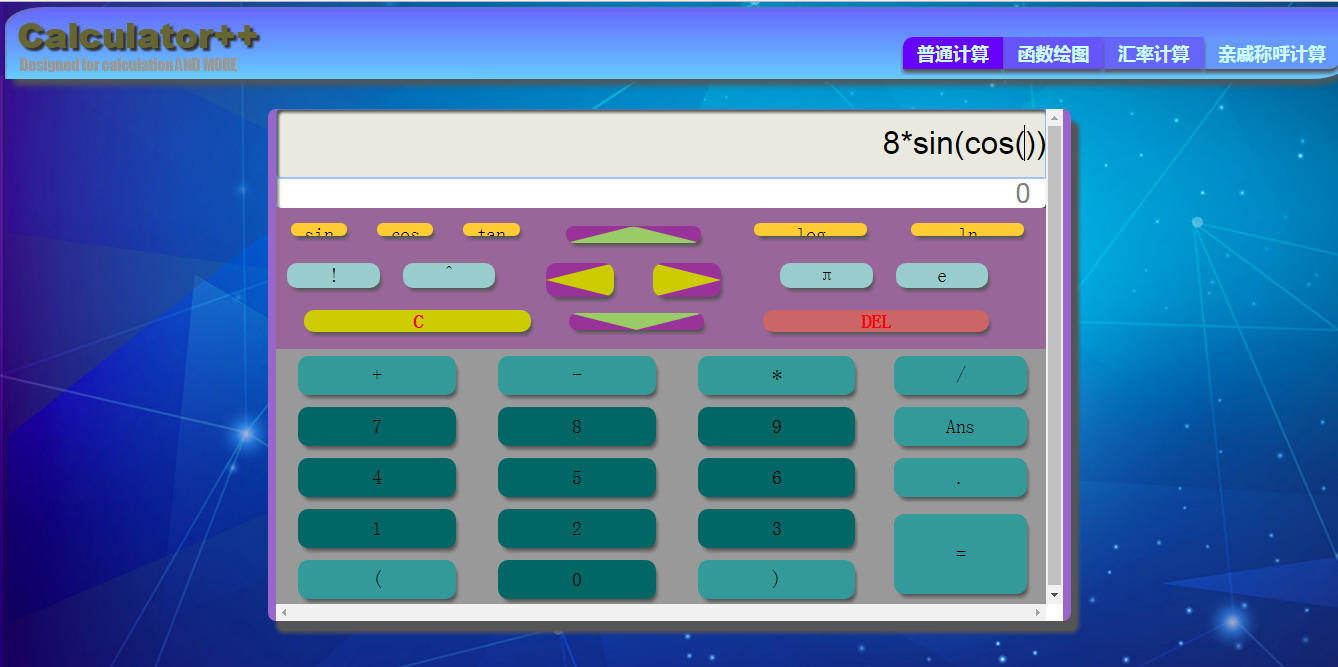
\includegraphics[width=5in]{cal.PNG}
\end{center}


在计算器中对于最简单的加减乘数四则运算是可以轻易算出答案的,因为通过JS的eval函数可以直接对其求值然后输出结果,而对于算式中包含像三角函数,阶乘,幂等符号或函数时就必须要先经过字符串处理,将其转化为eval可以直接执行的字符串,例如将sin转化为Math.sin,或π转化为Math.PI即可调用eval对其求值。所以Process就是按照这样的思路进行的。对于每个传给Process的参数,都会返回一个eval函数可以直接执行的字符串,这样计算器就可以支持包含这样字符的计算式了。

对于计算器的输入框,我们可以直接用键盘与鼠标进行操作,这是很简单的。而下面的一堆按钮通过button调用函数试想与键盘鼠标操作实现同样的通能。带有标志的button顾名思义,并且会在调用sin()这样带有括号的字符时,自动将光标定位到括号中,增加输入的流畅性。对于四个方向键,上下键代表了查阅历史记录,我们通过localStorage存储这些数据(每次按下等号时输入框所显示的内容),这样就可以实现刷新以及关闭浏览器,重新启动之后依然可以调用这两个按钮来获取历史信息。左右键则可以控制光标的移动,来利用按钮选择要输入的位置,但是由于点击需要一定的次数才可以达到目标位置,所以我建议用鼠标直接点击比较好。Ans键会在输入框的光标位置添加最近一次的答案数值。C键与Del键可以将输入框全部删除或删除光标位置前一个数字或字符。

\subsection{函数绘图}

在函数绘图中,我们接受从输入框获取的一个字符串,当用户点击确认按钮时,会调用Drawing函数,同时传入两个参数,前者为canvas的id,后者是图像的解析式,也就是从输入框中获取的数据,Process函数的实现主要就是将解析式分解为y和关于x的表达式,通过对大量的点被赋予x值以及利用与前面计算器相似的原理计算出y,得出大量的点的坐标,进而通过canvas的moveTo以及lineTo函数进行连线,而点的数量足够的多从而显示曲线足够光滑。另外值得注意的一点是,图像的坐标每个格为10个px,所以最好在函数的解析式中x乘上0.01,以及对右侧值乘上100可以得到较为清晰的图像。

效果如图:

\begin{center}
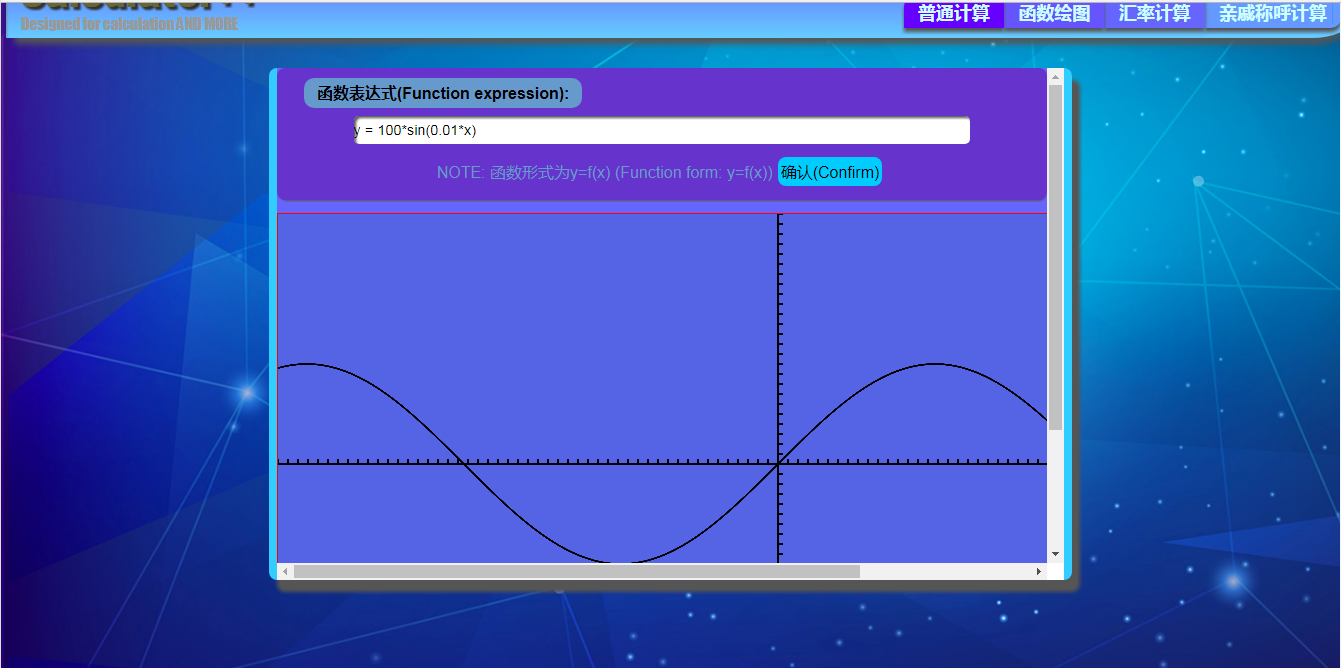
\includegraphics[width=5in]{func.PNG}
\end{center}

\subsection{实时汇率转换}

对于实时汇率转换,我们在NOWAPI网站上注册了一个账户,并且申请了免费试用调取汇率接口的权限,但可惜的是每个小时我们只能调用50次该接口,且使用时限也仅为1个月(使用时限是可以不断申请的)同样的,我们接受一个在输入框内的字符串代表要换算的金额,在下面的两个下拉栏中,我们可以选取174中货币,用户输入的金额代表的是源币种的数量,在用户点击确认之后,在下面一栏的结果中会显示以 "源币种数量 + 源币种代码 = 目标币种数量 + 目标币种代码" 的形式显示。由于使用权限是免费申请的,所以在非常小的概率下点击会过一段时间才会有结果的显示。 

另外,在本地自己测试时可以正常计算汇率,但是在GitHub Pages中不能正常使用。并且Github Pages中所显示的页面好像并不是实时的。

效果如图:

\begin{center}
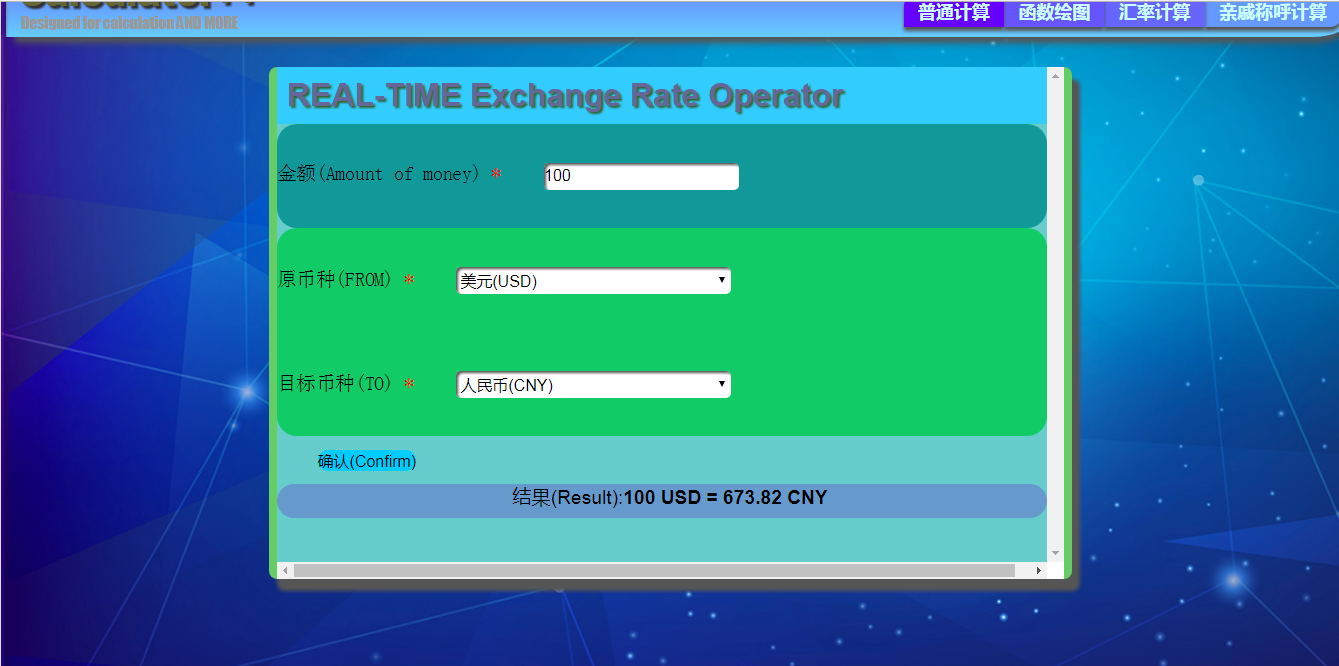
\includegraphics[width=5in]{rate.PNG}
\end{center}

\subsection{亲戚关系计算器}
由于亲戚关系的数据非常庞大,采用手动录入的方法所用的时间非常的长,现在只支持以只用"父亲的"或者"母亲的"向上查询,并加入了少量儿女及其下一代以及兄弟姐妹及其下一代的数据。目前的做法是将一个人直接的10种关系标号,1-父亲2-母亲3-丈夫4-妻子5-哥哥6-姐姐7-弟弟8-妹妹9-儿子10-女,然后用将关系编号以及关系名称以对象的形式存入数组,例如 'num':['99'],'salution': ['孙男'].这样存储.并在选择框内设置限制,男性不可能有丈夫以及父亲的儿子是不允许的。

效果如图:

\begin{center}
\includegraphics[width=5in]{rel1.PNG}
\end{center}

\subsection{历史记录}
已在计算器中说明了。


\newpage

\section{遇到的困难及解决方法}

\begin{enumerate}

\item
在调用汇率的接口时,不知道如何使用这个网址来获取数据,通过了解之后使用JQuery函数的ajax方法可以获得,这样之后确实可以获得其中数据并且在success时可以alert出来,但是无论如何相对一个变量赋值都是不行的,通过了解发现ajax这个函数时异步函数,他并不和下面的函数所在同一个线程之中,也就是说在下面调用ajax返回值赋值的时候可以ajax还没有请求到目标获取信息,所以赋值是不行的,。再然后发现网上都说在ajax里面将async设置为false,可以将ajax函数改为同步就可以进行赋值了,但是我再进行了这样的操作之后发现结果韩式不行,但是突然想到在success中既然可以alert出东西,那么我就不舍近求远了,就在其中直接加入document.getElementById.().innerHTML来修改结果的值之后发现成功了,在成功之后我也发现了在点击确认按钮时有时会过半秒钟才会有反应才体会到了请求是需要一定时间的。

\item
使用localStorage存储数据时,在W3School中的样例中感觉他每次都像在初始化localStorage中的东西,并加以输出,然后我就没有了解这个存储器的用法,后来想到可以通过判断该存储器中特定属性的属性值来判断是否已经被定义过,如果未被定义则初始化一个属性,若被定义了就用一个string数组来承载其属性值,便于在下面的代码中调用。


\end{enumerate}

\newpage

\section{心得感言}
我认为在进行前端设计的过程中,查阅资料是必不可少的,因为前端的一些主流操作是会变化的,同时,可能有一种你想实现的操作,自己费了九牛二虎之力才得以求解,但在网络上可能就会突然发现早就有人发表了更好的解决方案了,当然自己解决问题的过程是很重要的,不过能够学习其他人的高效率的方法也是对自己非常有益的。同时,可能CSS 或者 JS本身就带有某种方法,只不过我们还没有注意到,在通过查阅资料之后,就会体验到它的方便之处。在写JS代码过程中,往往会因为一些符号而导致错误,而js是一个新型的动态语言,他不会给我们报错,所以一定要养成一个不在这些细节上出错的习惯,在本次作业的完成中,我们就因为分号,或是逗号的缺失而导致代码无法执行,同时这些错误又很难察觉而导致尴尬的局面。同时在对一些变量名的问题上,我们尽量不要起那些意思明显而又有那么一丝可能会冲突的名字。在保存计算器的历史纪律中,我们组的一个人将保存历史记录的变量命名为history,就导致了已经写好的代码也无法正常运行的情况,之后才发觉冲突了。并且GitHub在组内合作时有很好的效果,保持实时更改代码以及管理代码的功能。


\end{document}